\documentclass[9pt]{beamer}

\input macros.tex

\title{Higher-level rules for sequent calculus}
\author[Miller, Pimentel]{
  \emph{Dale Miller} \\
  {\small Inria-Saclay \& Institut Polytechnique de Paris} \\[10pt]
  {\small Joint work with Elaine Pimentel, UCL} \\[20pt]
  {\small 6th International Workshop on Proof Theory, Birmingham}
}
\date{12 September 2024}

\begin{document}
\begin{frame}
	\titlepage
\end{frame}	


\begin{frame}{The original axioms-as-rules problem}

\begin{overlayarea}{\textwidth}{7cm}	
\only<1->{	
	How to incorporate \emphdr{inference rules} encoding axioms into existing proof systems 
	
	for \emphdb{classical and intuitionistic logics}?
}

\only<2-3>{
\medskip

\emphdb{Gentzen:} Add mathematical theories to first-order logic.

\begin{center}
{\em Consistency of the arithmetic without complete induction.}
\end{center}

\begin{tabular}{lcl}
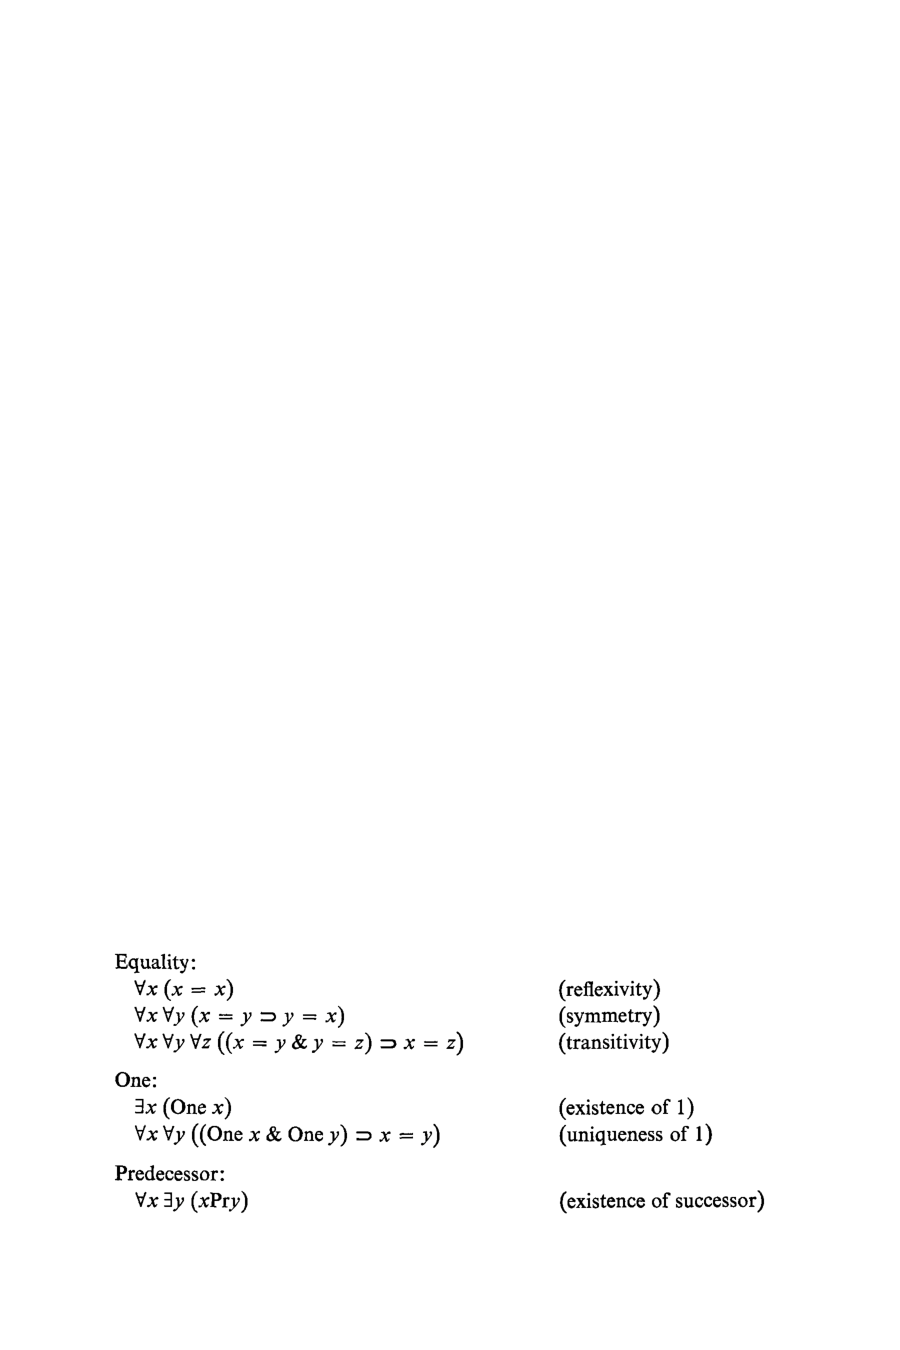
\includegraphics[scale=0.5]{figs/gentzen1} &\qquad& 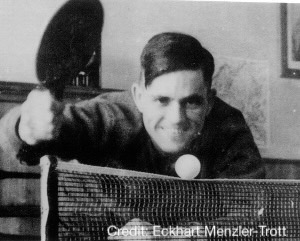
\includegraphics[scale=0.3]{figs/gentzen3}\\
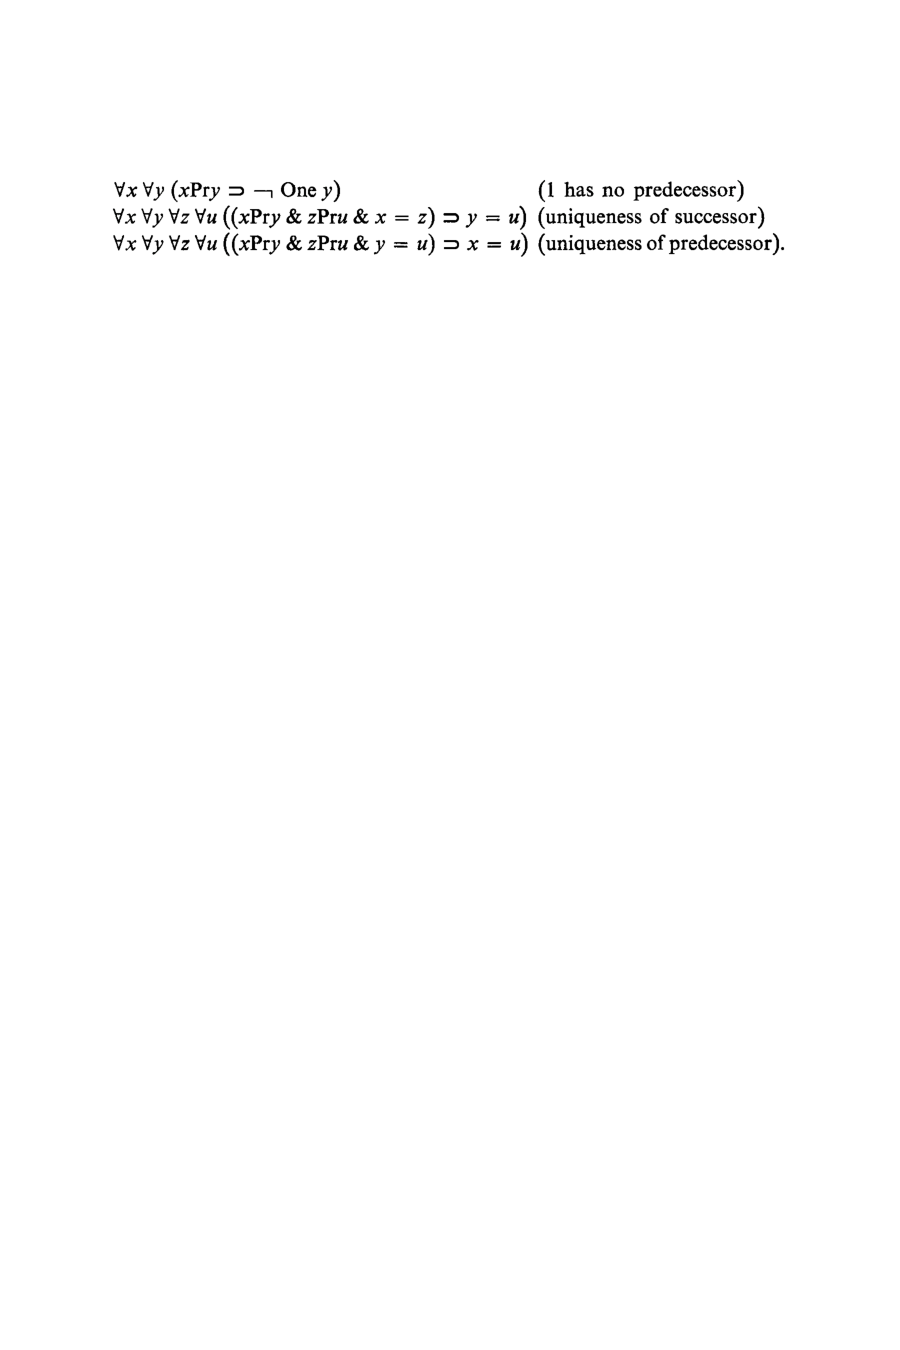
\includegraphics[scale=0.5]{figs/gentzen2} 
\end{tabular}
}	
\only<3>{
\begin{center}
{\em ``If our arithmetic is inconsistent, there exists a [cut-free] $\LK$ derivation with endsequent
\[
\mathfrak{U}_1,\ldots \mathfrak{U}_n\seq
\] 
where $\mathfrak{U}_1,\ldots \mathfrak{U}_n$ are arithmetic axiom formulae.''}
\end{center}
}


\only<4-5>{
\medskip

\emphdo{A naive attempt:} Add non-logical axioms.

\medskip

Assume $\vdash P\impl Q$ and $\vdash P$. 
			Then\semiproofadjust
			$$
			\infer[cut]{\vdash Q}
			{\infer{\vdash P}{}&
				\infer[cut]{P\vdash Q}
				{\infer{\vdash P\impl Q}{}&
					\infer[\impl_l]{P,P\impl Q\vdash Q}
					{\infer{P\vdash P}{}&
						\infer{Q\vdash Q}{}}}}
			$$
}
\only<5>{
\medskip

\emphdb{Girard}: The {\em Hauptsatz} fails for systems with proper axioms.}

\only<6-7>{
\medskip

\emphdo{A better approach:} Add non-logical rules of inference


\medskip
			
			$$
			\infer[\emphdb{P\impl Q}]{\Gamma, P\seq C}{\Gamma, Q\seq C}\qquad
			\infer[\emphdb{P}]{\Gamma\seq C}{\Gamma, P\seq C}
			$$
		}	
		
		\only<7>{
						The sequent $\seq Q$ now has the (cut-free) proof\semiproofadjust
			$$
			\infer[\emphdb{P}]{\seq Q}{\infer[\emphdb{P\impl Q}]{P\seq Q}
				{\infer{Q\seq Q}{}}}
			$$
		}
\end{overlayarea}
\end{frame}

\section{Polarisation}
\begin{frame}
\frametitle{Polarities of connectives}

\textbf{{Polarization is a feature of linear logic: $\otimes$, $\&$,
    $\oplus$, $\parr$}}
\begin{itemize}
  \item If the right-introduction rule is invertible, the connective
    is \negf{negative}.
  \item If the left-introduction rule is invertible, the connective
    is \posf{positive}.
  \item De Morgan duality flips polarity.  Polarity for atoms is
    assigned arbitrarily.
\end{itemize}
\vfill
\pause

\textbf{First-order classical and intuitionistic language:}
$$A\coloncolonequals P(x) \mid A \wedge A \mid t \mid A \vee A 
        \mid f \mid A \impl A \mid \exists x\, A \mid \forall x\, A$$
\vfill

\textbf{{Polarized connectives:}}
\begin{itemize}
\item In \emphdr{classical  logic}%, the \emph{polarized connectives} are:
\begin{itemize}
\item \posf{positive} and \negf{negative} versions of the logical connectives and constants: 
\[\wedgen, \wedgep, \truen, \truep,\veen, \veep, \falsen, \falsep\]
\end{itemize}
\item In \emphdr{intuitionistic logic} 
\begin{itemize}
\item polarized classical connectives and constants where $\falsen,\veen$ do not occur;
\item \negf{negative} implication: $\impl$.
\end{itemize}
\item First-order quantifiers: $\forall$ \negf{negative} and $\exists$ \posf{positive}.
\item A formula is \posf{positive} if it is a positive atom or has a
top-level positive connective.
\item A formula is \negf{negative} if it is a
negative atom or has a top-level negative connective.
\end{itemize}
\end{frame}

\begin{frame}{A fresh view to an old problem}

\begin{overlayarea}{\textwidth}{7cm}			
 \only<1->{Combining the \emphdb{polarities' hierarchy} [Ciabattoni et
     al., 2008] with a}
 \only<1>{\medskip
          \begin{center}
          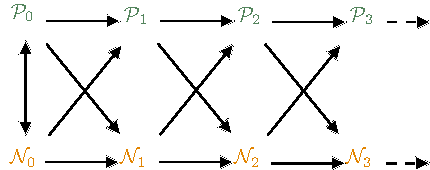
\includegraphics[scale=0.8]{figs/h5}
          \end{center}}
 \only<1>{\[\hbox{e.g., if $B$ is in $\posf{{\mathcal P}_0}$ then }
            \forall x\exists y\forall z. B\hbox{ is in }\negf{{\mathcal N}_3}.\]
  \medskip
  {\small $(\forall x\posf{P_1}\wedgen\posf{P_2})\wedgen(\forall y{B(y)}\wedgen \posf{P_3})$}
  \qquad
  \parbox[c]{2.5cm}{
     \scalebox{.65}{
       \begin{tikzpicture}[sibling distance=7em,level distance=4ex, level 2/.style={sibling distance =4em}]
           \node (neg 1) {$\wedgen$\strut}
		child { node {\rlap{$\wedgen$}\phantom{$\vee$}}
			child { node {$\forall$}
				child[level distance=3ex] {node[itria] {\smash{\posf{$P_1$}}}}}
			child {
					child[level distance=1ex] {node[itria] {\smash{\posf{$P_2$}}}}}}
			child { node {\rlap{$\wedgen$}\phantom{$\vee$}}
				child { node {$\forall$}
					child[level distance=5.5ex] {node {${B(y)}$}}}
				child {
					child[level distance=1ex] {node[itria] {\smash{\posf{$P_3$}}}}}};
      \end{tikzpicture}}}
   $\qquad\bm\rightarrow\quad$
	\parbox[c]{2.5cm}{
	\scalebox{.65}{
		\begin{tikzpicture}[sibling distance=4em,level distance=3.2ex]
		\node[ellipse,draw = orange,fill = orange!10] (neg2) {\negf{$\mathsf{neg}$}}
		child {
			child [level distance=-1ex]{node[itria] {\smash{\posf{$P_1$}}}}}
		child {
			child [level distance=-1ex]{node[itria] {\smash{\posf{$P_2$}}}}}
		child [level distance=6ex]{node {{$B(y)$}}}
		child {
			child [level distance=-1ex]{node[itria] {\smash{\posf{$P_3$}}}}};
		\end{tikzpicture}}}
  \medskip
  \begin{center}
  \emphdr{Bipolar} = $\mathcal{N}_2$\\
  (polarities flip at most twice)
  \end{center}}

\only<2->{
\medskip
systematic construction of synthetic rules from axioms using
\emphdb{focusing} [Andreoli, 1992],}
\only<2->{\medskip\emph{justifies} the introduction of the class of
          \emphdr{bipolar axioms}. Here, $B\in\mathcal{N}_2$.}
\only<2>{
\medskip
	\begin{tikzpicture}
	\node at (-1.9,2.6) {$\jUnf{\Gamma,B,\Gamma_1}{\cdot}{\cdot}{\Delta_1}\,\cdots\,\jUnf{\Gamma,B,\Gamma_n}{\cdot}{\cdot}{\Delta_n}$};
	\node at (-1.5,-1.4) {$\infer[\kern -2pt D_l]{
			\jUnf{\Gamma,B}{\cdot}{\cdot}{\Delta}}{
			\jLf{\Gamma,B}{B}{\Delta}}$};
	\node at (0,0) {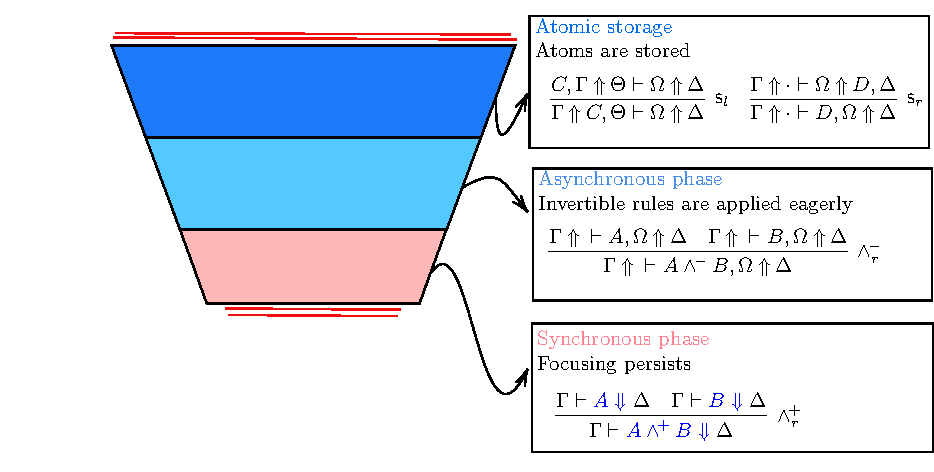
\includegraphics[scale=0.65]{figs/focusing}};
		\end{tikzpicture}}
\only<3>{\medskip
\begin{tikzpicture}
	\node at (-1.9,2.6) {$\jUnf{\Gamma,B,\Gamma_1}{\cdot}{\cdot}{\Delta_1}\;\ldots\;\jUnf{\Gamma,B,\Gamma_n}{\cdot}{\cdot}{\Delta_n}$};
	\node at (-1.5,-1.4) {$\infer[\kern -2pt D_l]{
			\jUnf{\Gamma,B}{\cdot}{\cdot}{\Delta}}{
			\jLf{\Gamma,B}{B}{\Delta}}$};
        \node at (-2.2,0.7) {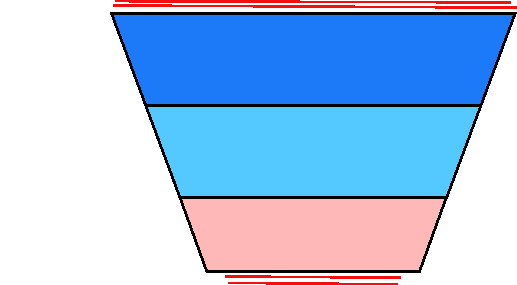
\includegraphics[scale=0.65]{figs/focusing2}};
	\node at (4,1) {\textbf{Corresponding synthetic rule}};
	\node at (4,0.5) {(in $\LK$ or $\LJ$)};
	\node at (4,-0.5) {
          $\infer[B]{\Gamma\seq\Delta}
                    {\Gamma,\Gamma_1\seq\Delta_1\quad\ldots\quad\Gamma,\Gamma_n\seq\Delta_n}$};
\end{tikzpicture}}
\end{overlayarea}
\only<2-3>{If $\Gamma\subseteq\mathcal{N}_{n}$  then
$\Gamma_i\subseteq\mathcal{N}_{n-2}$, for all $i=1,\ldots,n$.}
\end{frame}

\begin{frame}
\frametitle{The main results [Marin, Miller, Pimentel \& Volpe, 2022]}	
	
	\begin{block}{}
		\textbf{Theorem 1.} 
		Synthetic rules built from bipolar ($\mathcal{N}_2$) axioms 
                \emph{involve only atomic formulas}.
	\end{block}
	
	\bigskip
	
	\begin{block}{}
		\textbf{Theorem 2.} 
		The cut rule is admissible in the extension of $\LK/\LJ$ with 
                synthetic rules corresponding to bipolar axioms.
	\end{block}


\end{frame}

%\section{The roadmap}
%
%\begin{frame}\frametitle{Obtaining rules from axioms}
%	
%	\scalebox{.8}{
%		\begin{tikzpicture}
%		\tikzstyle{operation}=[->,>=latex,thick]
%		\tikzstyle{state}=[rectangle,draw,thick, rounded corners=5pt, text width = 1.6cm, align=center]
%		\tikzstyle{etiquette}=[rectangle,draw,thick,dotted]
%		%%rectangles
%		%\draw [fill=red!20, thick] (5,-0.5) rectangle (8,-3.5);
%		%\draw [fill=blue!20, thick, rounded corners=7pt] (-1.5,-0.5) rectangle (1.5,0.5);
%		%%points
%		\uncover<1->{
%			\node[state, fill=gray!20] (i) at (0,0)  {Unpolarized\\Axiom};
%		}
%		\only<1,12>{
%			\node[right = of i] {$\forall x (((P_1(x) \impl P_2(x)) \wedge Q(x)) \impl\exists y R(x,y))$};
%		}
%		%
%		\uncover<2->{
%			\node[state, fill=blue!20] (ii) at (2.5,2) {Polarized\\Axiom};
%			\node[state, fill=blue!20] (ii') at (2.5,-2) {Polarized\\Axiom};
%			%	\draw[dotted,thick] (2.5,1.2)--(2.5,-1.2);
%		}
%		%
%		\uncover<2->{
%			\draw[operation] (i)--(ii) node[etiquette] at (0.7,1.2) {Polarizing};
%			\draw[operation] (i)--(ii');
%		}
%		\only<2-5,9,11>{
%			\draw[operation,dotted] (i)--(2,0.8);
%			\draw[operation,dotted] (i)--(2,0);
%			\draw[operation,dotted] (i)--(2,-0.8);
%		}
%		%
%		\only<2-4>{
%			\node[right] at (2,0.8) {$\negf{\bm\forall}x (((\posf{P_1}(x) \negf{\bm\impl} \negf{P_2}(x)) \posf{\bm\wedgep} \posf{Q}(x)) \negf{\bm\impl}\posf{\bm\exists}y \posf{R}(x,y))$};
%		}
%		\only<2-3,9>{
%			\node[right] at (2,0) {$\negf{\bm\forall}x (((\posf{P_1}(x) \negf{\bm\impl} \negf{P_2}(x)) \negf{\bm\wedgen} \negf{Q}(x)) \negf{\bm\impl}\posf{\bm\exists}y \posf{R}(x,y))$};
%		}
%		\only<2-3,11>{
%			\node[right] at (2,-0.8) {$\negf{\bm\forall}x (((\posf{P_1}(x) \negf{\bm\impl} \negf{P_2}(x)) \negf{\bm\wedgen} \posf{Q}(x)) \negf{\bm\impl}\posf{\bm\exists}y \posf{R}(x,y))$};
%		}
%		%
%		\uncover<3->{
%			\node[etiquette] at (4.5,3) {Is it bipolar?};
%		}
%		%
%		\uncover<4-8,9-10,12>{
%			\draw[thick] (ii)--(4.5,2) node[circle,draw,fill=green!40] {$\bm\checkmark$};
%		}
%		\uncover<11-12>{
%			\draw[thick] (ii')--(4.5,-2) node[circle,draw,fill=red!40] {$\bm\times$};%node[etiquette] 
%		}
%		%
%		\uncover<5-8,10,12>{
%			\node[state, fill=green!20] (iii) at (6.5,2) {Bipole\\in \LKF}; 
%			\draw[operation] (4.85,2)--(iii);
%		}
%		\only<5-7>{
%			\node[] at (8.5,-0.5) {$
%				\infer[\forall_l]{\jLf{\Gamma}{\negf{\bm\forall}x (((\posf{P_1}(x) \negf{\bm\impl} \negf{P_2}(x)) \posf{\bm\wedgep} \posf{Q}(x)) \negf{\bm\impl}\posf{\bm\exists}y \posf{R}(x,y))}{}{\Delta}}{
%					\infer[\impl_l]{{\jLf{\Gamma}{((P_1(t) \impl P_2(t)) \wedgep Q(t)) \impl \exists y R(t,y)}{}{\Delta}}}{
%						\infer[\wedgep_r]{\jRf{\Gamma}{(P_1(t) \impl P_2(t)) \wedgep Q(t)}{\Delta}}{
%							\infer[\krelease_r]{{\jRf{\Gamma}{P_1(t)\impl P_2(t)}{\Delta}}}{
%								\infer[\impl_r]{\jUnf{\Gamma}{\cdot}{P_1(t)\impl P_2(t)}{\Delta}}{
%									\infer[\kstore_l]{\jUnf{\Gamma}{P_1(t)}{P_2(t)}{\Delta}}{
%										\infer[\kstore_r]{\jUnf{\Gamma,P_1(t)}{\cdot}{P_2(t)}{\Delta}}{
%											\deduce{\jUnf{\Gamma,\posf{P_1(t)}}{\cdot}{\cdot}{\negf{P_2(t)},\Delta}}{}
%										}
%									}
%								}
%							} 
%							& 
%							\infer[\kinit_r]{\jRf{\Gamma}{\posf{Q(t)}}{\Delta}}{}
%						} 
%						& 
%						\infer[\krelease_l]{\jLf{\Gamma}{\exists y R(t,y)}{\Delta}}{
%							\infer[\exists_l]{\jUnf{\Gamma}{\exists y R(t,y)}{\cdot}{\Delta}}{
%								\infer[\kstore_l]{\jUnf{\Gamma}{R(t,z)}{\cdot}{\Delta}}{
%									\deduce{\jUnf{\Gamma, \posf{R(t,z)}}{\cdot}{\cdot}{\Delta}}{}
%								}
%							}
%						}
%					}
%				}
%				$};
%		}
%		%
%		\uncover<7-12>{
%			\node[state, fill=orange!20] (iv) at (9.5,2) {Inference\\rule for \LK};
%		}
%		\uncover<6-8,12>{
%			\draw[operation] (iii)--(iv) node[etiquette] at (8,3) {Synthesizing};
%		}
%		\only<7-8>{
%			\node[draw] at (11,1) {$
%				\infer[]{\Gamma = \Gamma', \emphdr{Q(t)}\seq\Delta}{
%					\Gamma, \emphdr{P_1(t)}\seq\emphdr{P_2(t)},\Delta
%					& 
%					\Gamma, \emphdr{R(t,z)}\seq\Delta}
%				$};
%		}
%		%
%		\only<10>{
%			\node[draw] at (10.5,1) {$
%				\infer[]{\Gamma\seq\Delta}{
%					\Gamma, \emphdr{P_1(t)}\seq\emphdr{P_2(t)},\Delta
%					&
%					\Gamma \seq\emphdr{Q(t)},\Delta
%					& 
%					\Gamma, \emphdr{R(t,z)}\seq\Delta}
%				$};
%		}
%		%
%		\only<12>{
%			\node[draw] at (11.5,0) {$
%				\infer[]{\Gamma = \Gamma', \emphdr{Q(t)}\seq\Delta}{
%					\Gamma, \emphdr{P_1(t)}\seq\emphdr{P_2(t)},\Delta
%					& 
%					\Gamma, \emphdr{R(t,z)}\seq\Delta}
%				$};
%			\node[draw] at (10.5,-1.5) {$
%				\infer[]{\Gamma\seq\Delta}{
%					\Gamma, \emphdr{P_1(t)}\seq\emphdr{P_2(t)},\Delta
%					&
%					\Gamma \seq\emphdr{Q(t)},\Delta
%					& 
%					\Gamma, \emphdr{R(t,z)}\seq\Delta}
%				$};
%		}
%		\end{tikzpicture}
%	}
%	
%	
%\end{frame}





\section{Examples}
%\subsection{Geometric axioms}
%
%\begin{frame}\frametitle{Geometric axioms as bipoles}
%	
%\only<1>{\emphdr{Geometric implication:}}
%%
%\only<2->{\emphdo{Polarized geometric implication:}}
%		
%%\begin{overlayarea}{\textwidth}{1cm}
%\only<1>{
%		\[\forall \overline{z} (P_1 \wedge \ldots \wedge P_m \, \impl \, \exists \overline{x}_1 M_1 \vee \ldots \vee \exists \overline{x}_n M_n ) 
%		\]
%}	
%\only<2>{
%\[\negf{\forall \overline{z}} (P_1^{\pm} \wedgepn \ldots \wedgepn P_m^{\pm} \, \negf{\impl} \, \posf{\exists \overline{x}_1} \hat{M_1} \veepn \ldots \veepn \posf{\exists \overline{x}_n} \hat{M_n} )
%		\]
%}
%\only<3>{
%	$$
%	\negf{\forall \overline{z}} (\posf{P_1^{+}} \posf{\wedgep} \ldots \posf{\wedgep} \posf{P_m^{+}} \, \negf{\impl} \, \posf{\exists \overline{x}_1} \hat{M_1} \veepn \ldots \veepn \posf{\exists \overline{x}_n} \hat{M_n} ) \, ,
%	$$
%}
%\only<4>{
%	$$
%	\negf{\forall \overline{z}} (\negf{P_1^{-}} \wedgepn \ldots \wedgepn \negf{P_m^{-}} \, \negf{\impl} \, \posf{\exists \overline{x}_1} \hat{M_1} \veepn \ldots \veepn \posf{\exists \overline{x}_n} \hat{M_n} ) \, ,
%	$$
%}
%%\end{overlayarea}
%
%\bigskip
%
%\begin{overlayarea}{\textwidth}{4cm}
%\only<1>{
%\begin{itemize}
%	\item $P_i$ atomic;
%	\item $M_j=Q_{j_1}\wedge\ldots\wedge Q_{j_{k_{j}}}$, $Q_{j_k}$ atomic; 
%	\item none of the variables in the vectors $\overline{x}_j$ are free in $P_i$.
%\end{itemize}	
%}
%\only<2>{
%\begin{itemize}
%\item $\posf{P_i^+}, \negf{P_i^-}$ atomic;
%\item $\hat{M_j} = Q_{j_1}^{\pm} \posf{\wedgep} \ldots \posf{\wedgep} Q_{j_{k_{j}}}^{\pm}$ , $Q_{j_k}^{\pm}$ atomic;
%\item none of the variables in the vectors $\overline{x}_j$ are free in $P_i$.
%\end{itemize}
%}		
%\only<3>{
%		\emph{Corresponding bipole}:	
%		$$\infer{\jUnf{\emphdr{\overline{P}},\Gamma'}{\null}{\null}{\Delta}}
%		{\jUnf{\emphdr{\overline{Q}_1[\overline{y}_1/\overline{x}_1]},\Gamma}{\null} {\null}{\Delta} & \ldots & \jUnf{\emphdr{\overline{Q}_n[\overline{y}_n/\overline{x}_n]},\Gamma}{\null} {\null}  {\Delta}}
%		$$
%		with $\overline{P}=\{\posf{P_i^+}\}, \overline{Q_j}=\{Q_{j_k}^\pm\}$. 
%
%		\bigskip
%				
%		\emphdb{Corresponding $\LK$ rule}:	
%		$$\infer[GRS]{\emphdr{\overline{P}},\Gamma'\vdash \Delta}
%		{\emphdr{\overline{Q}_1[\overline{y}_1/\overline{x}_1]},\Gamma\vdash\Delta & \ldots & \emphdr{\overline{Q}_n[\overline{y}_n/\overline{x}_n]},\Gamma\vdash\Delta}
%		$$
%	}
%	
%	\only<4>{
%		\emph{Corresponding bipole}:	
%		$$\infer[m+n\mbox{ premises}]{\jUnf{\Gamma}{\null}{\null}{\Delta}}
%		{\jUnf{\emphdr{\overline{Q}_j[\overline{y}_j/\overline{x}_j]},\Gamma}{\null} {\null}{\Delta} & \ldots &\jUnf{\Gamma}{\null} {\null}{\emphdr{P_i},\Delta} }
%		$$
%with $\overline{Q_j}=\{Q_{j_k}\}$. 
%
%		\bigskip
%				
%		\emphdb{Corresponding $\LK$ rule}:	
%		$$\infer[m+n\mbox{ premises}]{\Gamma\vdash \Delta}
%		{\emphdr{\overline{Q}_j[\overline{y}_j/\overline{x}_j]},\Gamma\vdash \Delta & \ldots & \Gamma\vdash \emphdr{P_i},\Delta}
%		$$		
%		}
%\end{overlayarea}
%	
%\end{frame}


\begin{frame}\frametitle{\only<1-4>{Example: Horn clauses as bipoles} \only<5>{Other examples}}

\only<1>{\[
		\forall \overline{z}(P_1 \wedge \ldots \wedge P_m \, \impl \, Q)
		\]}
	
\only<2>{\[
		\negf{\forall \overline{z}}(P_1^{\pm} \wedgepn \ldots \wedgepn P_m^{\pm} \, \negf{\impl} \, Q^{\pm})
		\]}
	
\only<3>{\[
	\negf{\forall \overline{z}}(\posf{P_1^{+}} \posf{\wedgep} \ldots \posf{\wedgep} \posf{P_m^{+}} \, \negf{\impl} \, \posf{Q^{+}} )
	\]}

\only<4>{\[
	\negf{\forall \overline{z}}(\negf{P_1^{-} \wedgen} \ldots \negf{\wedgen P_m^{-}} \, \negf{\impl} \, \negf{Q^{-}})
	\]}
		
\bigskip


\begin{overlayarea}{\textwidth}{2cm}
\only<3>{
$$	\infer[FC]
	{\emphdr{\overline{P}}, \Gamma'\vdash\Delta}
	{\emphdr{Q}, \Gamma\vdash\Delta}	
	$$
\begin{center}
\emph{Forward-chaining} \\
\emph{[Simpson, Negri, Ciabattoni]}
\end{center}
}

\only<4>{
$$\infer[BC]
	{\Gamma\vdash \emphdr{Q},\Delta'}
	{\Gamma\vdash \emphdr{P_1}, \Delta & \ldots &\Gamma\vdash \emphdr{P_m}, \Delta}
	$$
\begin{center}
\emph{Back-chaining}\\
\emph{[Vigan\`o]}
\end{center}
}
\only<5>{
\begin{center}
Geometric, co-geometric, universal axioms...
\end{center}
\medskip
\[\negf{\forall \overline{z}} (P_1^{\pm} \wedgepn \ldots \wedgepn P_m^{\pm} \, \negf{\impl} \, \posf{\exists \overline{x}_1} \hat{M_1} \veepn \ldots \veepn \posf{\exists \overline{x}_n} \hat{M_n} )
		\]
		\smallskip
\[
		\negf{\forall \overline{z}} (\negf{\forall \overline{x}_1} \hat{M_1} \wedgepn \ldots \wedgepn \negf{\forall \overline{x}_n} \hat{M_n}  \, \negf{\impl} \, \negf{P_1^{-} \veen} \ldots \negf{\veen P_m^{-}} ) 
		\]
		\smallskip
\[
		\negf{\forall \overline{z}}(P_1^{\pm} \wedgepn \ldots \wedgepn P_m^{\pm} \, \negf{\impl} \, Q_1^{\pm} \veepn \ldots \veepn Q_n^{\pm})
		\]
}
\end{overlayarea}
\end{frame}


\begin{frame}
\frametitle{Recapitulation}

\begin{itemize}

\item \textbf{Polarity of connectives:} invertibility vs
  non-invertibility of introduction rules\\[10pt]

\item \textbf{Focusing:} uses polarity to organize proofs into a
  two-phase structure.\\[10pt]

  These features of proofs arose within linear logic.  The \LKF and
  \LJF proof systems apply these features to classical and
  intuitionistic logics.  [Liang \& Miller, 2009]\\[10pt]

\item \textbf{Synthetic inference rules:}
\pause
  \begin{itemize}
  \item \textbf{Bipoles:} A flexible means exists to translate bipoles
    ($\mathcal{N}_2$) to inference rules involving only atomic
    formulas: see [Marin, Miller, Pimentel, \& Volpe, 2022].\\[6pt]
\pause

  \item \textbf{Non-bipoles:} The topic of the rest of this talk. Two
    approaches:
    \begin{itemize}
    \item Transform non-bipoles into bipoles.
    \item Use a higher-level system of rules.
    \end{itemize}
  \end{itemize}

\end{itemize}

\end{frame}


\begin{frame}
\frametitle{One approach to treating non-bipoles: Remove them}

Transform non-bipolar formulas into bipolar formulas by introducing
new predicate symbols.

\begin{itemize}
\item Tseitin [1960's], Mints et al.~[1982].
\item Andreoli: skolemization [1992], bipolarization [2001].
\item Dyckhoff \& Negri: geometrisation [2015]
\item See Dyckhoff \& Negri for many other names and references.
\end{itemize}

\vfill\pause
With higher-order quantification, provability can be maintained.
\[
  u\impl ((p\impl q)\impl r) \impl s \dashv\vdash {\color{red}\exists x. }
\left(\begin{array}{c}
    (u\impl(x\impl r) \impl s)~\wedge~\\
    (x\impl (p\impl q))~\wedge~\\
    ((p\impl q)\impl x)
\end{array}
\right)
\]
\pause
If you drop $\exists x$ for a new predicate symbol, the expressions
are equisatisfiable.

\newcommand{\sledom}{\Relbar\joinrel\mathrel{|}}

\[
  u\impl ((p\impl q)\impl r) \impl s \sledom \models
\left(\begin{array}{c}
    (u\impl (x\impl r) \impl s) \wedge~\\
    (x\impl (p\impl q))  \wedge~\\
    ((p\impl q)\impl x)
\end{array}
\right)
\]
\vfill
N.B.: With only implications, $B$ is of order $n$ if and only if $B\in\mathcal{N}_n$.
\vfill
\end{frame}

\begin{frame}
\frametitle{Another approach to treating non-bipoles: Higher-level of rules}

Let $C$ denote $u\impl ((p\impl q)\impl r) \impl s$.  (Assume that
$s$ has negative polarity.)

\[
  \infer{\jUnf{\Gamma, C}{\cdot}{\cdot}{s}}{
  \infer={\jLf{\Gamma, C}{u\impl ((p\impl q)\impl r) \impl s}{s}}{
    \infer[\krelease_r]{\jRf{\Gamma,C}{u}}{
       \infer[\kstore_l]{\jUnf{\Gamma,C}{\cdot}{u}{\cdot}}
                        {\jUnf{\Gamma,C}{\cdot}{\cdot}{u}}}
& 
  \infer[\krelease_l]{\jRf{\Gamma,C}{(p\impl q)\impl r}}{
  \infer{\jUnf{\Gamma,C}{\cdot}{(p\impl q)\impl r}{\cdot}}{
  \infer{\jUnf{\Gamma,C}{p\impl q}{r}{\cdot}}{
\jUnf{\Gamma,C,p\impl q}{\cdot}{\cdot}{r}
}}}
& 
    \infer[\kinit_l]{\jLf{\Gamma,C}{s}{s}}{}
}}
\]
This justifies the synthetic inference rule
\[
  \infer[C]{\Gamma\seq s}{ \Gamma\seq u & \Gamma,p\impl q \seq r}
\]
Unfortunately, this contains an occurrence of a logical connective.
\vfill
The $\mathcal{N}_1$ formula $p\impl q$ formula can be
replaced by an inference rule: which rule depends on polarity.
\vfill
\end{frame}

\begin{frame}
\frametitle{Higher-level of rules: an example}

The synthetic rule for $C=u\impl ((p\impl q)\impl r) \impl s$ (where 
$s$ has negative polarity).
\[\left[\quad\vcenter{
  \infer[C]{\Gamma\seq s}{\Gamma\seq u
   \quad &\quad
   \infer{\Gamma\seq r}{
     \deduce{\strut\vdots}{
     \left(\vcenter{\hbox{Rule based on $p\impl q$}}\right)}}}
}\quad\right]\]
The second premise has an inference rule that is
available to prove that premise.\pause  The shape of that rule depends on 
the polarity of $p$ and $q$.  There are four possibilities.
\[\qquad
  \infer[(p-,~q-)]{\Psi\seq q}{\Psi\seq p}
  \qquad 
  \infer[(p-,~q+)]{\Psi\seq E}{\Psi\seq p & \Psi,q \seq E}
\]
\[
  \infer[(p+,~q-)]{\Psi,p\seq q}{}
  \qquad 
  \infer[(p+,~q+)]{\Psi,p\seq E}{\Psi,p, q \seq E}
\]
For example,
\[\left[\quad\vcenter{
  \infer[C]{\Gamma\seq s}{\Gamma\seq u
   \quad &\quad
   \infer{\Gamma\seq r}{
     \deduce{\strut\vdots}{
     \left(\vcenter{\infer{\Psi,p\seq E}{\Psi,p, q \seq E}}\right)}}}
  }\quad\right]
\]
\end{frame}

\newcommand{\Twoseq}[3]{{\color{darkred}#1:}\,#2\vdash #3}
\newcommand{\LUB}{\textsf{\color{blue}lub}}
\newcommand{\lub   }[3]{\LUB~#1~#2~#3}

\begin{frame}
\frametitle{Higher-level of rules: An example with quantifiers}

The (polarized) formula stating the existence of least upper bounds.
\[
  \forall x\forall y\exists z(x\le z\wedgep y\le z\wedgep
              \forall w(x\le w\wedgep y\le w\impl z\le w)),
\]
Focusing on this formula yields the derivation.
\[
  \infer
        {\Twoseq{\Sigma}{\Gamma}{\Delta}}
        {\Twoseq{\Sigma,z}
                {\forall w(x\le w\wedgep y\le w\impl z\le w),~
                   x\le z,~y\le z,~\Gamma}
                {\Delta}}
\]
Sequents are prefixed with a list of eigenvariables $\Sigma$ which are
bound over the sequent.
\vfill\pause

The assumption $\forall w(x\le w\wedgep y\le w\impl z\le w)$ can be
converted to an inference rule (depending on the polarity of the $\le$
predicate).  For example,
\[
  \infer{\Twoseq{\Sigma}{\Gamma}{\Delta}}
        {\infer{\Twoseq{\Sigma,z}{\Gamma,x\le z,~y\le z}{\Delta}}
               { \deduce{\strut\vdots}{
     \left(\vcenter{
  \infer{\Twoseq{\Sigma,z}{\Gamma}{z\le w}}
        {\Twoseq{\Sigma,z}{\Gamma}{x\le w} \qquad
         \Twoseq{\Sigma,z}{\Gamma}{y\le w}}
     }\right)}}}
\]
There are no logical constants.  The \emph{scope} of variables is
getting complicated.
\end{frame}

\begin{frame}
\frametitle{Higher-level of rules: Continued}

The $\mathcal{N}_3$ formula\quad
\[
  \forall x\forall y\exists z(x\le z\wedgep y\le z\wedgep
              \forall w(x\le w\wedgep y\le w\impl z\le w)),
\]
can be bipolarized by introducing a new predicate \LUB\xspace so that
the atomic formula $(\lub{x}{y}{z})$ denotes the fact that $z$ is the
least upper bound of $x$ and $y$. 
\[
  \begin{array}{c}
   \forall x\forall y\exists z.[ (x\le z\wedgep y\le z\wedgep\lub{x}{y}{z})]
   \wedgen~\\[6pt]
   \forall x\forall y\forall z.[ \lub{x}{y}{z}\equiv \forall w.(x\le w\wedgep y\le w\impl z\le w)]
  \end{array}
\]
\vfill

Focusing on this formula yields the derivation.
\[
  \infer
        {\Twoseq{\Sigma}{\Gamma}{\Delta}}
        {\Twoseq{\Sigma,z}
                {\lub{x}{y}{z},~x\le z,~y\le z,~\Gamma}
                {\Delta}}
\]
%Now, sequents are prefixed with a list of eigenvariables that are
%bound over the sequent.
\vfill

It seems more natural to use this formulation with a new predicate
than the rule with a new scoped inference rule.
\vfill

Note: If the order relation is also known to be antisymmetric, then
the \textsf{lub} predicate actually defines a function.  Moving from 
relations to functions is another topic.

\end{frame}

\begin{frame}
\frametitle{Higher-level of rules in natural deduction}

If we limit ourselves to
\begin{itemize}
  \item negative connectives ($\impl$, $\wedge^-$,
    $\forall$) and
    \item negative polarized atoms,
\end{itemize}
then the sequent calculus is essentially natural deduction:
[Herbelin 1994],\\[0pt] [Esp{\'{\i}}rito Santo 2007].

\vfill

Systems of higher-level rules in natural deduction have been
considered long ago.

\begin{itemize}
\item Schroeder-Heister, A Natural Extension of Natural
  Deduction, 1984.

\item Avron, Gentzenizing Schroeder-Heister's Natural Extension of
  Natural Deduction, 1990.

\item  Harper, Honsell, Gordon Plotkin, "A Framework for Defining
  Logics", 1993.
\end{itemize}
\end{frame}

\begin{frame}
\frametitle{Higher-level of rules in sequent calculus}

Using the papers [Marin, Miller, Pimentel, \& Volpe, 2022] and [Miller
  \& Pimentel, 2013], we should be able to describe systems of
higher-level rules for the sequent calculus that accounts for
\begin{itemize}
\item intuitionistic, classical, linear proof systems,
\item additive and multiplicative connectives,
\item forward-chaining and back-chaining polarities, and 
\item first-order quantification and eigenvariables.
\end{itemize}
\vfill
\pause

However: Capturing these features without using logical connectives
seems a questionable pursuit since logical formulas have evolved to
capture all these features (except for the polarity of atoms).
\vfill

\begin{itemize}
\item The implications $\multimap$, $\Rightarrow$ do not 
  have natural counterparts in inference rules.
  
\item The nesting of scopes for quantifiers ($\forall$, $\exists$) is
  natural in logical formulas, while writing explicit binders in
  inference rules is eschewed.
\end{itemize}
\vfill

\end{frame}

\begin{frame}
\frametitle{Future plans}

\begin{itemize}

\item We plan to consider how higher-level rules can be organized to
  capture the richness of inference in the sequent calculus for (at
  least) classical, intuitionistic, and linear logics.

\vfill

\item We will need to understand the trade-offs between bipolarizing
  formulas (with the introduction of new predicates) or not.
  \medskip
  
\begin{itemize}
  \item Developing these approaches in an interactive theorem
    prover (such as Abella) might provide an interesting setting to
    explore these trade-offs in various simple mathematical theories.
\end{itemize}
\vfill

\item We also hope to understand the relations between higher-level
  rules and more “exotic” proof systems: hypersequents [Ciabattoni \&
    Genco, 2018]. 
\vfill
\vfill
\end{itemize}
\end{frame}

\end{document}

% LocalWords:  Ciabattoni itria FC Vigan bipolarization darkred lub
% LocalWords:  geometrisation bipolarized antisymmetric rito Avron
% LocalWords:  Gentzenizing Heister's Honsell bipolarizing Genco
